\documentclass[12pt]{article}
\usepackage{ctex}
\usepackage[english]{babel}
\usepackage{blindtext}
\usepackage{nameref}
\usepackage{fancyhdr}
\usepackage{amsmath,amssymb,amsthm}
\usepackage{graphicx,float}
\usepackage{physics}
\usepackage{pgfplots}
\usepackage[a4paper, total={6in, 9in}]{geometry}

\graphicspath{{../image/}}

\pagestyle{fancy}
\fancyhf{}
\fancyhf[HL]{極限}
\fancyhf[CF]{\thepage}

\newcommand{\innerprod}[2]{\langle{#1},{#2}\rangle}
\newcommand{\id}{\mathtt{id}}

\newtheorem{definition}{定義}
\newtheorem*{theorem}{定理}
\newtheorem*{corollary}{衍理}
\newtheorem*{lemma}{引理}
\newtheorem*{proposition}{設理}
\newtheorem*{remark}{小記}
\newtheorem*{claim}{主張}
\newtheorem*{example}{例子}
\newtheorem*{axiom}{公設}
\renewenvironment*{proof}{\textit{證明.}}{\hfill$\qed$}

\newenvironment*{sol}{\par \textbf{解}.}{\hfill$\blacksquare$}

\begin{document}
    \section*{無窮小量與無窮大量}
    
    在高等數學,對於無窮的討論,一般從無窮小量開始。何爲無窮小量?即一個非常接近0的變量不斷向零靠近,而永遠無法到達0,即爲無窮小量。

    我們可以考慮數列$\{a_n\}$, 其中對於任意整數$n$,$a_n=\dfrac{1}{10^n}$。則當$n$越大時,$a_n$越靠近0。對此,記$$a_n\to 0$$考慮對任意$n$,均有$\varepsilon>0$使得$0<\varepsilon<a_n$,則稱變量$\varepsilon$為無窮小量。記$\varepsilon\to 0$。

    相對的,考慮數列$\{A_n\}$, 其中對於任意整數$n$,$A_n=10^n$。則當$n$越大時,$A_n$越靠近$\infty$。對此,記$$A_n\to \infty$$考慮對任意$n$,均有$N>0$使得$A_n<N$,則稱變量$N$為無窮大量。記$N\to \infty$。

    由此發現,無窮小量與無窮大量互相關聯:

    \begin{axiom}
        若$a_n=\dfrac{1}{A_n}$,則$$\lim_{A_n\to \infty}a_n=0$$ 
    \end{axiom}

    以上亦可簡記為$\displaystyle\lim_{x\to\infty}\frac{1}{x}=0$.

    \section*{極限的幾何概念}

    想象一個漩渦,然後有一個點$p$在漩渦裏漂浮,其結果就是\textbf{$p$會不斷沿著漩渦中心繞圈,無限接近漩渦中心,但永遠不會到達中心}。此刻,我們稱$p$所走的路綫為$p$的\textbf{軌跡},記$p(t)$並以$t>0$作時間變數,而漩渦中心$p_0$則爲$p$的軌跡的極限,記$$p_0=\lim_{t\to\infty}p(t)$$

    \begin{figure}[H]
        \centering
        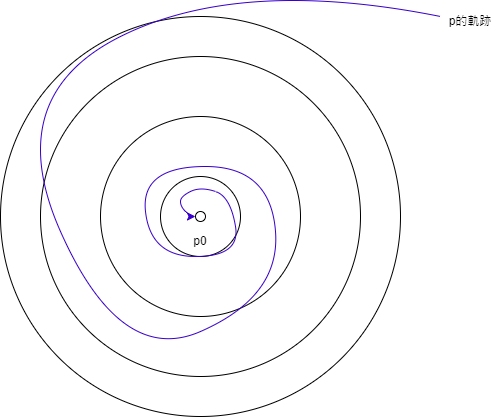
\includegraphics[scale=0.4]{limit1.png}
    \end{figure}    

    留意上圖,$p$的軌跡從外圍開始,不斷趨近於$p_0$。可見對於任何圓心為$p_0$且半徑爲$r>0$的圓形,均有$p(t)$位於圓形内。我們稱$p(t)$的極限\textbf{收斂};反之,若$p(t)$沒有唯一極限(甚至沒有極限),我們稱之爲\textbf{發散}。

    那麽,該如何證明極限收斂性成爲了微分數學一個重要命題。對此,幾何學家定名了一個數學模型,稱爲\textbf{賦距空間},指一個數學空間中,擁有計算距離的函數:

    \begin{definition}[距離函數]
        對於一個數集$S$,若函數$d:S\times S\to\mathbb{R}$符合以下條件:\begin{itemize}
            \item (正定性)對於任何$x,y\in S$,均有$d(x,y)\geq 0$;$d(x,y)=0$當且僅當$x=y$。
            \item (對稱性)對於任何$x,y\in S$,$d(x,y)=d(y,x)$。
            \item (三角不等式)對於任何$x,y,z\in S$,$d(x,z)\leq d(x,y)+d(y,z)$。
        \end{itemize}
        則稱$d$為$S$的距離函數。
    \end{definition}

    \begin{definition}[賦距空間]
        設$d$為數集$S$的距離函數,則稱$(S,d)$為賦距空間。
    \end{definition}

    \begin{example}
        若$d(x,y)=\sqrt{(x-y)^2}:\mathbb{R}\times\mathbb{R}\to \mathbb{R}$,則$(\mathbb{R},d)$為賦距空間。

        \begin{proof}
            證明函數$d$符合距離公式條件:
            \begin{enumerate}
                \item 正定性:$d(x,y)=\sqrt{(x-y)^2}\geq \sqrt{0}=0$。同時$$d(x,y)=0\iff (x-y)^2=0\iff x-y=0\iff x=y$$
                \item 對稱性:$d(x,y)=\sqrt{(x-y)^2}=\sqrt{(y-x)^2}=d(y,x)$。
                \item 三角不等式:\begin{align*}
                    [d(x,z)]^2&=(x-z)^2\\
                    &=(x-y+y-z)^2\\
                    &=(x-y)^2+2(x-y)(y-z)+(y-z)^2\\
                    &\leq [d(x,y)]^2+2[d(x,y)][d(y,z)]+[d(y,z)]^2\\
                    &=[d(x,y)+d(y,z)]^2
                \end{align*}
            \end{enumerate}
            因此,$d$為$\mathbb{R}$上的距離公式,$(\mathbb{R},d)$為賦距空間。
        \end{proof}
    \end{example}

    \begin{remark}
        此距離為絕對值函數$|\cdot|$。
    \end{remark}

    \begin{example}
        設$x=(x_1,x_2),y=(y_1,y_2)$。若$d(x,y)=\sqrt{(x_1-y_1)^2+(x_2-y_2)^2}:\mathbb{R}^2\times\mathbb{R}^2\to \mathbb{R}$,則$(\mathbb{R}^2,d)$為賦距空間。
        \begin{figure}[H]
            \centering
            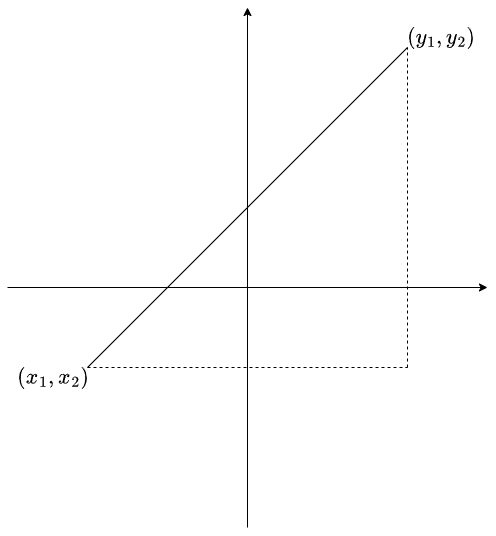
\includegraphics[scale=0.6]{EuclideanDistance.png}
            \caption{歐氏幾何:$\mathbb{R}^2=\mathbb{R}\times\mathbb{R}$即xy坐標平面}
        \end{figure}

        \begin{proof}
            證明函數$d$符合距離公式條件:
            \begin{enumerate}
                \item 正定性:$d(x,y)=\sqrt{(x_1-y_1)^2+(x_2-y_2)^2}\geq \sqrt{0}=0$。同時$$d(x,y)=0\iff (x_1-y_1)^2+(x_2-y_2)^2=0\iff \begin{cases}
                    x_1-y_1=0\\
                    x_2-y_2=0
                \end{cases}\iff x=y$$
                \item 對稱性:$d(x,y)=\sqrt{(x_1-y_1)^2+(x_2-y_2)^2}=\sqrt{(y_1-x_1)^2+(y_2-x_2)^2}=d(y,x)$。
                \item 三角不等式:證明留作習題。
            \end{enumerate}
            因此,$d$為$\mathbb{R}^2$上的距離公式,$(\mathbb{R}^2,d)$為賦距空間。
        \end{proof}
    \end{example}

    \begin{remark}
        此距離為歐式距離函數,亦稱通常距離。
    \end{remark}

    在正規數學當中,無論是在一維、二維、三維,還是更高維的賦距空間,我們都希望擁有極限收斂。利用距離公式定義收斂性,可讓我們對收斂性有更直觀的判斷。現定義於賦距空間$(S,d)$上$p$點的\textbf{$\varepsilon$-鄰域}為$$U_\varepsilon(p):=\{q\in S:d(p,q)<\varepsilon\}$$

    \begin{definition}[聚點]
        設$x(t)$為軌跡,若有$x_0$令任何$\varepsilon>0$,均有$x(t)\in U_\varepsilon(x_0)$,則$x_0$為$x(t)$的聚點。
    \end{definition}

    \begin{definition}[聚點(2)]
        設$(x_n)$為一系列點,若有$x_0$令任何$\varepsilon>0$,均有$x_n\in U_\varepsilon(x_0)$,則$x_0$為$x_n$的聚點。
    \end{definition}

    \begin{definition}[極限收斂]
        設$x_0$為$(x_n)$的聚點,而且對於任何$n>0$,均有$\varepsilon>0$使得所有$m> n$都有$x_m\in U_\varepsilon(x_0)$,則稱$x_0$為$(x_n)$的極限,或$(x_n)$收斂於$x_0$。
    \end{definition}

    \begin{example}
        設$x_n:=\dfrac{1}{n}$,則$(x_n)$在$(\mathbb{R},|\cdot|)$收斂於$0$,$\lim_{n\to \infty}x_n=0$。

        \begin{proof}
            對於任意$n>0$,均可設$\varepsilon=\frac{1}{n}$使得當$m> n$時$$d(x_m,0)=\frac{1}{m}<\frac{1}{n}=\varepsilon$$
        \end{proof}
    \end{example}

    \section*{$\varepsilon-\delta$定義-於無窮小的極限}
    \section*{極限的性質}
    \section*{特殊的極限}
    \section*{於無窮大的極限}
    \section*{連續函數}
    \section*{連續函數的性質}
    \section*{介值定理}
    \section*{單調函數與逆函數}
\end{document}